%%%%%%%%%%%%%%%%%%%%%%%%%%%%%%%%%%%%%%%%%%%%%%%%%%%%%%%%%%%%%%%%%%%%%%%%
%    INSTITUTE OF PHYSICS PUBLISHING                                   %
%                                                                      %
%   `Preparing an article for publication in an Institute of Physics   %
%    Publishing journal using LaTeX'                                   %
%                                                                      %
%    LaTeX source code `ioplau2e.tex' used to generate `author         %
%    guidelines', the documentation explaining and demonstrating use   %
%    of the Institute of Physics Publishing LaTeX preprint files       %
%    `iopart.cls, iopart12.clo and iopart10.clo'.                      %
%                                                                      %
%    `ioplau2e.tex' itself uses LaTeX with `iopart.cls'                %
%                                                                      %
%%%%%%%%%%%%%%%%%%%%%%%%%%%%%%%%%%
%
%
% First we have a character check
%
% ! exclamation mark    " double quote  
% # hash                ` opening quote (grave)
% & ampersand           ' closing quote (acute)
% $ dollar              % percent       
% ( open parenthesis    ) close paren.  
% - hyphen              = equals sign
% | vertical bar        ~ tilde         
% @ at sign             _ underscore
% { open curly brace    } close curly   
% [ open square         ] close square bracket
% + plus sign           ; semi-colon    
% * asterisk            : colon
% < open angle bracket  > close angle   
% , comma               . full stop
% ? question mark       / forward slash 
% \ backslash           ^ circumflex
%
% ABCDEFGHIJKLMNOPQRSTUVWXYZ 
% abcdefghijklmnopqrstuvwxyz 
% 1234567890
%
%%%%%%%%%%%%%%%%%%%%%%%%%%%%%%%%%%%%%%%%%%%%%%%%%%%%%%%%%%%%%%%%%%%
%

%AIP Reprint Class%%%%%%%%%%%%%%%%%%%%%%%%%%%%%%%%%%%%%%%%%%%%%%%%%%%%%%%%%%%%%%%%%%%%%%%%%%%%%
\documentclass[aip,prl,amsmath,amssymb,reprint,superscriptaddress]{revtex4-1} %preprint version
\usepackage{graphicx}% Include figure files
\usepackage{dcolumn}% Align table columns on decimal point
\usepackage{bm}% bold math
\usepackage{epstopdf}

    \renewcommand{\topfraction}{0.9}    % max fraction of floats at top
    \renewcommand{\bottomfraction}{0.8}    % max fraction of floats at bottom
    \setcounter{topnumber}{2}
    \setcounter{bottomnumber}{2}
    \setcounter{totalnumber}{4}     % 2 may work better
    \setcounter{dbltopnumber}{2}    % for 2-column pages
    \renewcommand{\dbltopfraction}{0.9}    % fit big float above 2-col. text
    \renewcommand{\textfraction}{0.07}    % allow minimal text w. figs
    \renewcommand{\floatpagefraction}{0.7}    % require fuller float pages
    \renewcommand{\dblfloatpagefraction}{0.7}    % require fuller float pages
    \setlength{\abovecaptionskip}{5pt}
    \setlength{\belowcaptionskip}{5pt}
    \setlength{\parskip}{0pt}
    \setlength{\textfloatsep}{5pt} 

%%%%%%%%%%%%%%%%%%%%%%%%%%%%%%%%%%%%%%%%%%%%%%%%%%%%%%%%%%%%%%%%%%%%%%%%%%%%%%%%%%%%%%%%%%%%%%%%%%

%IOP preprint class %%%%%%%%%%%%%%%%%%%%%%%%%%%%%%%%%%%%%%%%%%%%%%%%%%%%%%%%%%%%%%%%%%%%%%%%%%%%%%
%\documentclass[12pt]{iopart}
%\newcommand{\gguide}{{\it Preparing graphics for IOP journals}}
%Uncomment next line if AMS fonts required
%\usepackage{iopams}
%\usepackage{graphicx}
%\usepackage{epstopdf}  
%%%%%%%%%%%%%%%%%%%%%%%%%%%%%%%%%%%%%%%%%%%%%%%%%%%%%%%%%%%%%%%%%%%%%%%%%%%%%%%%%%%%%%%%%%%%%%%%%%
%Slava's inserts %%%%%%%%%%%%%%%%%%%%%%%%%%%%%%%%%%%%%%%%%%%%%%%%%%%%%%%%%%%%%%%%%%%%%%%%%%%%%%
%\usepackage{amsfonts}
%\usepackage{amssymb}

%\newcommand{\ptt}[1]{\frac{\partial#1}{\partial t}}
%\newcommand{\vvec}{\mathbf{v}}
%\newcommand{\Bvec}{\mathbf{B}}
%\newcommand{\Evec}{\mathbf{E}}
%\newcommand{\Jvec}{\mathbf{J}}
%\newcommand{\Avec}{\mathbf{A}}
%%%%%%%%%%%%%%%%%%%%%%%%%%%%%%%%%%%%%%%%%%%%%%%%%%%%%%%%%%%%%%%%%%%%%%%%%%%%%%%%%%%%%%%%%%%%%%%%%%

\begin{document}
\title{Observation of turbulent intermittency scaling with magnetic helicity in an experimental MHD plasma}

\author{D.A. Schaffner}
\affiliation{Swarthmore College, Swarthmore, PA, USA}
\author{A. Wan}
\affiliation{Swarthmore College, Swarthmore, PA, USA}
\author{M.R. Brown}
\affiliation{Swarthmore College, Swarthmore, PA, USA}
\date{\today}
\begin{abstract}
The intermittency in turbulent magnetic field fluctuations has been observed to scale with the amount of magnetic helicity injected into an experimentl flux rope plasma. A selectively decayed Taylor state is created in the wind-tunnel configuration of the Swarthmore Spheromak Experiment using a stuffed plasma gun. The amount of flux in the core of the gun can be varied linearly which in turn modfies the amount of helicity injected into the plasma. The level of intermittency is determined by finding the flatness (4th order moment) of the probability distribution function of increments for magnetic fluctuations. This higher order aspect of the turbulence is observed to increase with the injected helicity while the spectral index in the inertial range of the turbulence appears to be unaffected by this variation. Some experimental evidence is given for the role of current sheets and reconnection sites in the generation of this intermittency, but the true nature of the observed intermittency remains unknown.
\end{abstract}

\maketitle

The study of magnetic turbulence in laboratory experiment and in space plasmas has been conducted using a multitude of approaches including the construction and analysis of power spectra, correlations and probability distribution functions for both temporal and spatial datasets~\cite{deWit13}. Much focus has been placed on studying power spectra, or really, the rate of transfer of energy from large scales to small scales reflected in the spectral index, as this quantity has the most intuitive physical reason and firmest connection to the Kolmogorov theory of fluid turbulence. However, examination of power spectra follows only one thread of insight into the characteristics that make up a turbulent plasma. The role of intermittency in turbulence theory has developed alongside spectral theory in fluid mechanics~\cite{frisch95} and has become an integral aspect of turbulence analysis in both space~\cite{Greco08,Greco09,Wan09} and laboratory plasmas~\cite{carter06,serianni07}. 

This paper presents the results of an experimental scan which establishes a connection between a controllable experimental quantity---magnetic helicity---and a turbulent characteristic---intermittency---as well as highlights the need for a multi-pronged approach to turbulence analysis. The experimental scan was conducted on the wind-tunnel configuration of the Swarthmore Spheromak Experiment which consists of a 86cm long by 15.5cm wide cylindrical copper flux conserver into which a plasma gun (shown in Figure~\ref{fig:plasmagun_closeup2} injects dense, highly magnetized ($\sim 1\times 10^{15} cm^{-3}, \sim 5kG$) plasma which self-organizes into a Taylor state~\cite{Gray13}. The injected magnetic helicity of the plasma can be modified by setting the amount of flux through the plasma gun using a coxial magnetic coil. Power spectra and probability density functions of increments are constructed using fluctuation magnetic data extract from pickup coils ($\dot{B}$ probes) inserted radially into the flux conserver at the midplane. While power-law fits to the power spectra show no scaling with the change in helicity, the turbulent intermittency, as indicated by the calculated flatness of the PDFs, increases with the helicity with flatness values ranging from near Gaussian (F$\sim 5$) to values over 30.

%In a laboratory plasma, Gray, {\it et al.}~\cite{Gray13} recently reported on the observation of a long-lived helical flux rope called a Taylor double-helix in the SSX MHD wind tunnel.  The Taylor double-helix is the natural relaxed state of MHD plasma confined in a long, perfectly conducting cylinder~\cite{Taylor86}.  In the case of an infinite cylinder of radius $a$, the minimum energy state has a helical pitch of $ ka = 1.234$, where k is the wave number associated with the axis of the cylinder.

%In the SSX experiments, a magnetized plasma gun launches a magnetized plasma plume into a long flux conserving cylinder.  The plasma rapidly relaxes to the double-helix state in about 1 Alfv\'en crossing time and subsequently decays resistively.  Gray, {\it et al.}~\cite{Gray13} postulated that the physics of selective decay was at play as the initially turbulent plasma relaxed to the double-helix state.  The selective decay hypothesis posits that the energy selectively decays relative to the magnetic helicity because the energy spectra peaks at higher wave numbers, where dissipation is higher~\cite{Matthaeus80}.  The wind tunnel's minimum energy state possesses $ka = 1.292$, which is within 5\% of the infinite cylinder's $ka = 1.234$. 

\begin{figure}[!htbp]
\centerline{
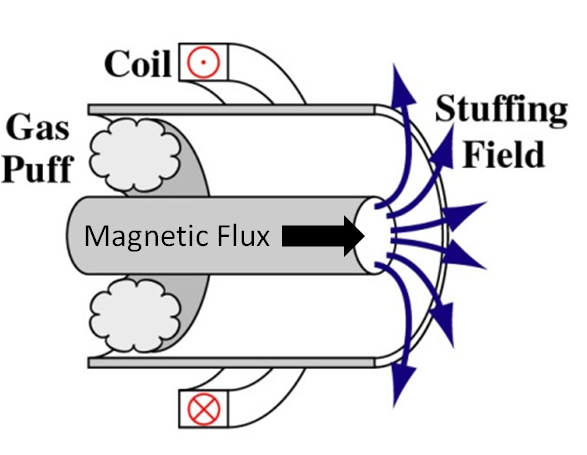
\includegraphics[width=8.5cm]{plasmagun_closeup2.png}}
\caption{\label{fig:plasmagun_closeup2} Diagram of the plasma gun attached to one end of the copper flux conserver in SSX. The diagram shows how the magnetic flux in the core of the gun is modifed by adjusting the current in the coil outside of the gun which sets up the stuffing field.}
\end{figure}

The injection of magnetic helicity into the plasma is a natural consequence of the formation procedure for a plasma gun. Magnetic helicity,
%
\begin{equation}
K_{B} = \int A \cdot B dV
\label{eq:helicity_th}
\end{equation}
%
is a measure of the amount of twistedness of the magnetic field lines and can be expressed in terms of magnetic flux squared (i.e. units of $Wb^{2}$). This quantity can be recast in a more experimentally relevant quantity, 
%
\begin{equation}
K_{B} = \int \Phi V_{gun} dt
\label{eq:helicity_exp}
\end{equation}
%
where $\Phi$ is the magnetic flux penetrating the plasma gun core and $V_{gun}$ is the voltage drop across the gun gap. This is the form of the helicity that is calculated and reported as in this paper. Since the plasma forms under the assumption of selective decay (conservation of magnetic helicity) are reported in Gray 2013[~\cite{Gray13}], it is further assumed that the amount of helicity injected by the gun is conserved and present in the plasma under observation. Though the voltage across the gun gap is recored for the entire duration of the shot, only the first $20 \mu s$ are used to estimate the injected helicity. Beyond $20 \mu s$, the voltage measurement is significantly affected by breaking fieldlines during spheromak formation. Though it is assumed that helicity injection is nearly constant for the duration of the discharge, the values of helicity reported here is that for the first $20 \mu s$ after the initial trigger.

\begin{figure}[!htbp]
\centerline{
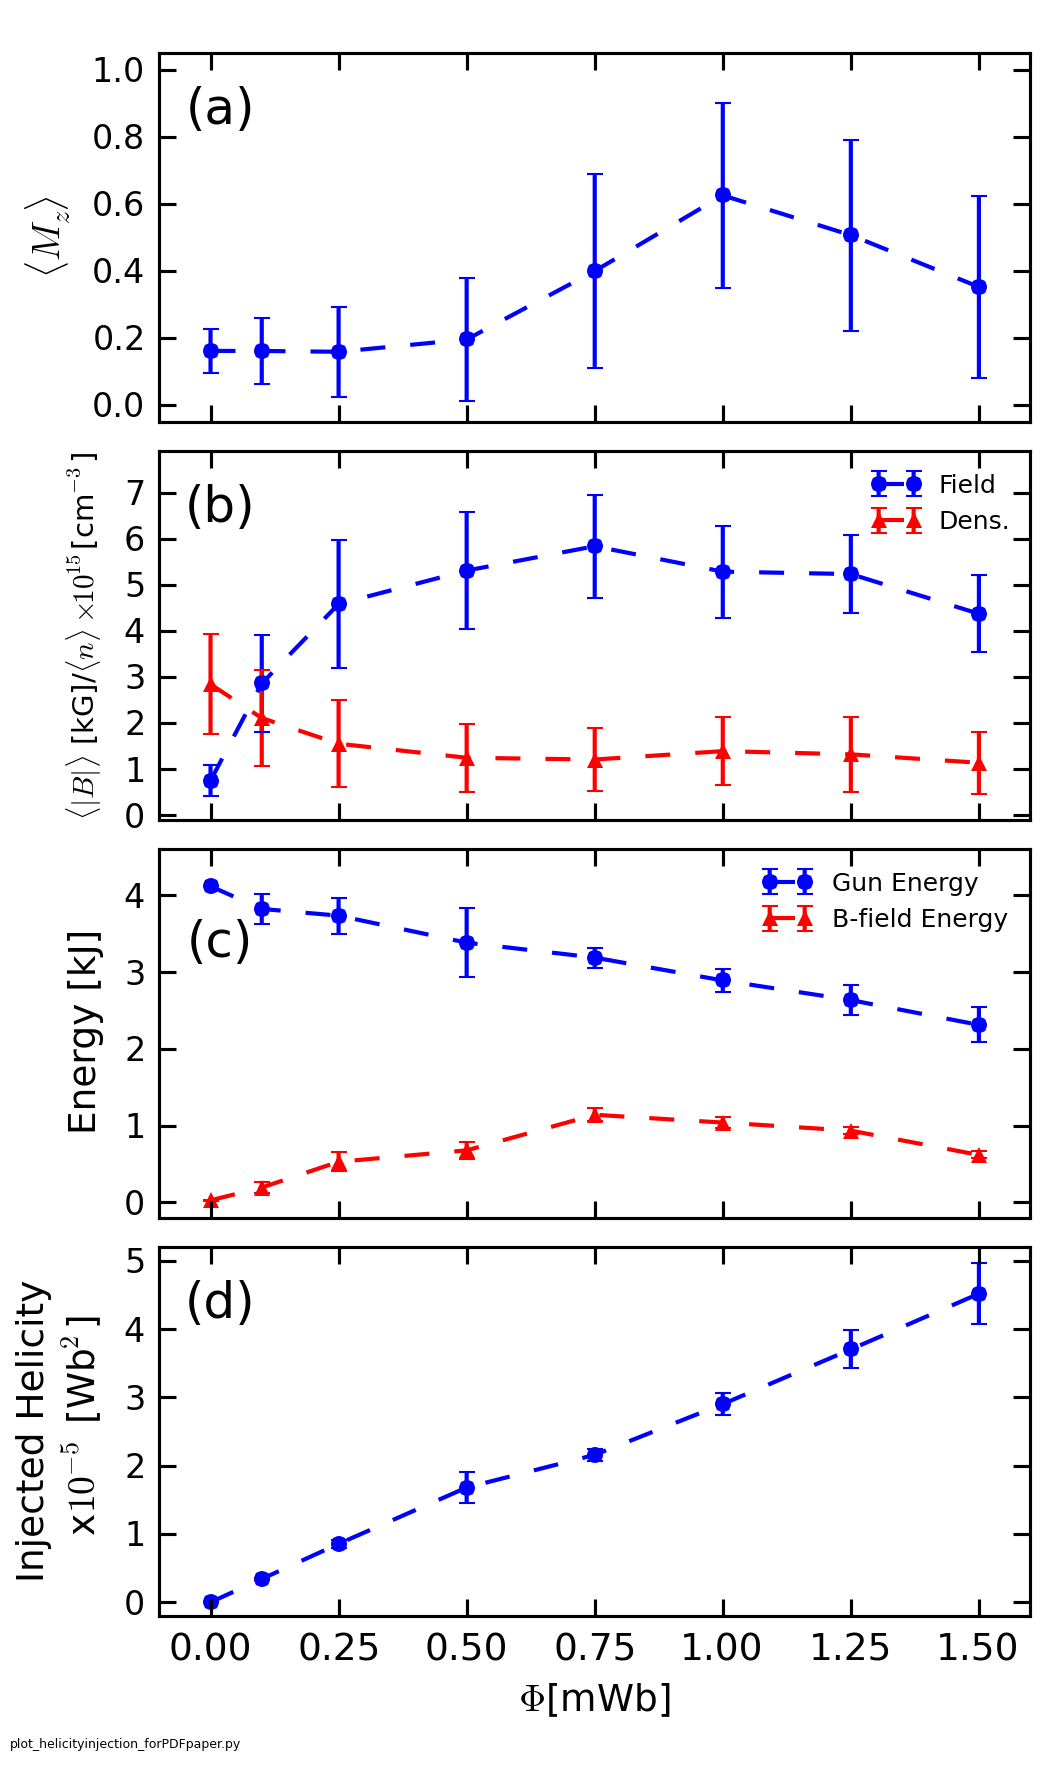
\includegraphics[width=8.5cm]{helicity_scaling.png}}
\caption{\label{fig:helicity_scaling} (a) Average magnetic field magnitude over the equilibrium epoch (40-60$\mu s$), (b) injected gun energy and volume integrated magnetic field energy, and (c) amount of helicity injected in the first $20 \mu s$ after discharge trigger as a function of magnetic flux in gun core.}
\end{figure}

The gun voltage is set by a combination of the gun circuit and breakdown physics, but typically does not vary given a particular capacitor charge setting and gas input delay time. Thus, by~\ref{eq:helicity_exp}, the injected helicity is modified by the amount of magnetic flux penetrating the gun core. This flux, in turn, is set by the the amount of current run through the stuffing coil. The stuffing coil produces magnetic field parallel to the gun axis using a capacitor discharge circuit, but with a much longer timescale than the gun discharge. Because the stuffing coil discharge is much slower, rather than modifity the discharge voltage to vary the magnetic field in the gun, the field is set by changing the timing of when the gun fires relative to the stuffing coil. Thus, changes in flux, and consquently helicity are adjusted by changing the timing delay of the gun trigger.

The amount of flux in the gun core is enhanced by the used of a Permadure? in within the gun core. This allows for the flux to be ranged from 0.0 to 1.5mWb which given a gun voltage of approximately 900V yields an injected helicity range of 0 to 5$x10^{-5} Wb^{2}$ for the first $20 \mu s$. As indicated in Figure~\ref{fig:helicity_scaling}(c), the injected helicity scales linearly with the varied magnetic flux. Figure~\ref{fig:helicity_scaling}(a) and (b) show how the average magnetic field in the center of the chamber and the energy changes with magnetic flux. The magnetic field is determined using a three-axis Bdot probe about 1cm off of the central cylindrical axis, and is time averaged from 40 to 60$\mu s$ which constitutes the equilibrium epoch of the discharge so called as it is the range of most time stationary fluctuations. As Figure~\ref{fig:helicity_scaling}(a) shows, this value increases initially with flux, but saturates at a value around $5kG$ for most flux settings. The gun energy is found by integrating the power, $P = I_{gun}V_{gun}$, from 0.0 to 60.0$\mu s$ and represents the maximum amount of energy that can be delivered into the plasma. This value begins around $4kJ$ which is about half of the possible circuit energy based on the 1mF, 4.0kV capacitor circuit, and decreases steadily with increasing flux as shown with blue in Fig.~\ref{fig:helicity_scaling}(b). The amount of energy that actually gets deposited into the magnetic fields is indicated by red in Fig.~\ref{fig:helicity_scaling}(b), and as would be expected, follows a similar trend as the field magnitude. This energy is calculated by finding the energy density, $B^{2}/2\mu_{0}$, for each Bdot tip, and integrating over the volume at each radially location.

The power spectrum of magnetic field fluctuations for each helicity case is presented in Figure~\ref{fig:Br_spectra}. The curves shown are constructed by taking the a sixth-order Morlet wavelet transform~\cite{torrence98} of each $\dot{B}_{r}$ timeseries and scaled to $B_{r}$ by diving through by frequency squared. Each curve shows a cascade of power from low frequencies to high frequencies, though the absolute scale in Figure~\ref{fig:Br_spectra}(a) has been artificially staggered in order to allow for each curve to be clearly seen. Each spectra exhibits a break-point around 1MHz; a power-law fit is made to the linear region around the break-point for each curve using a Maximum Likelihood Estimation method~\cite{clauset09}. The spectral index and error for each fit is indicated in Figure~\ref{fig:Br_spectra}. Though the helicity is increasing linearly, the power-law fit for each spectra does not change significantly, hovering around a slope of 3 for low frequency fits and around 5 for high frequency fits. This trend indicates that the change in helicity does not appear to have an effect on the cascade process from larger scales to smaller scales.

\begin{figure}[!htbp]
\centerline{
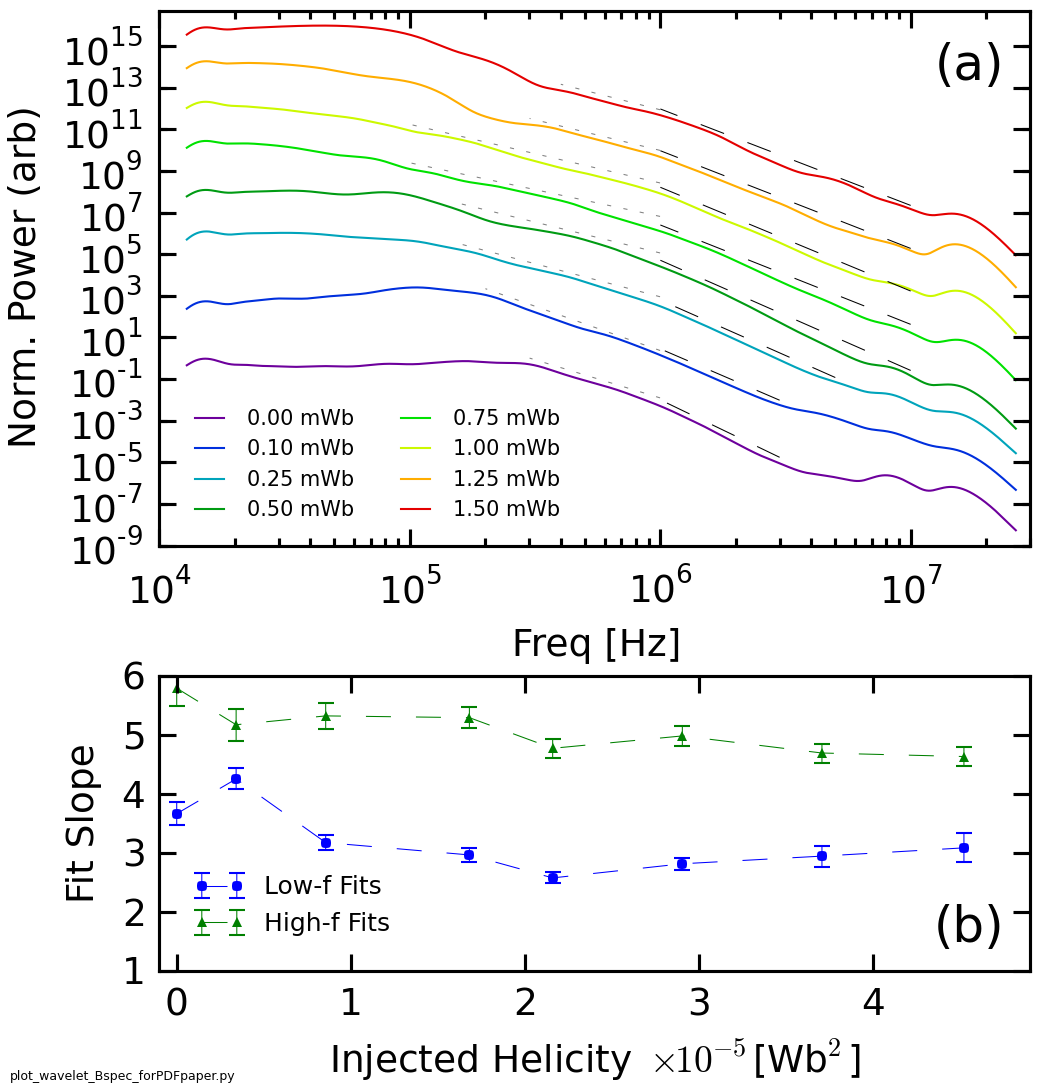
\includegraphics[width=8.5cm]{Br_spectra.png}}
\caption{\label{fig:Br_spectra} (a) Wavelet generated magnetic field fluctuation spectra for the radial direction ($B_{r}$), for each of the eight helicity states. The spectra are staggered in order to highlight the shape of each spectrum. (b) Fits for each spectra for either low or high frequencies. The width in frequency of each fit is indicated by the dashed lines in (a).}
\end{figure}

The amount of intermittency in the plasma for each helicity state does, however, appear to change. Figure~\ref{fig:Br_flatness} demonstrates how intermittency is determined through the measure of flatness. Fig.~\ref{fig:Br_flatness}(a) shows the probability distribution function of increments (PDF) of a timeseries at 2$\times 10^{-5}$ Wb$^{2}$ of injected helicity for two different timescales: $0.15\mu s$ and $15\mu s$. The PDF of increments is constructed by taking differences of values in a time signal---in this case, $\dot{B}_{r}$---separated by a time scale. As Fig.~\ref{fig:Br_flatness}(a) shows, the PDF with small time scale shows a highly pointed PDF with broad, fat tails indicating large excursions from the mean value---or intermittency. This non-Gaussian behavior is indicated by a best-fit Gaussian curve. The PDF with a large time scale increment clearly show a much more Gaussian distribution compared to its best fit. The level of intermittency for each scale can be quantified by taking the normalized fourth-order moment of the PDF---also called flatness or kurtosis. The flatness for each PDF at each times scale, as well as for each helicity state, is shown in Fig.~\ref{fig:Br_flatness}(b). Clearly, each state shows increasing flatness, and thus intermittency, with decreasing time scale. The flatness of a purely Gaussian distribution is indicated at F=3. Moreover, it is observed that the overall flatness of each curve increases as a function of helicity. In other words, the intermittency of the plasma appears to increase with injected helicity.

\begin{figure}[!htbp]
\centerline{
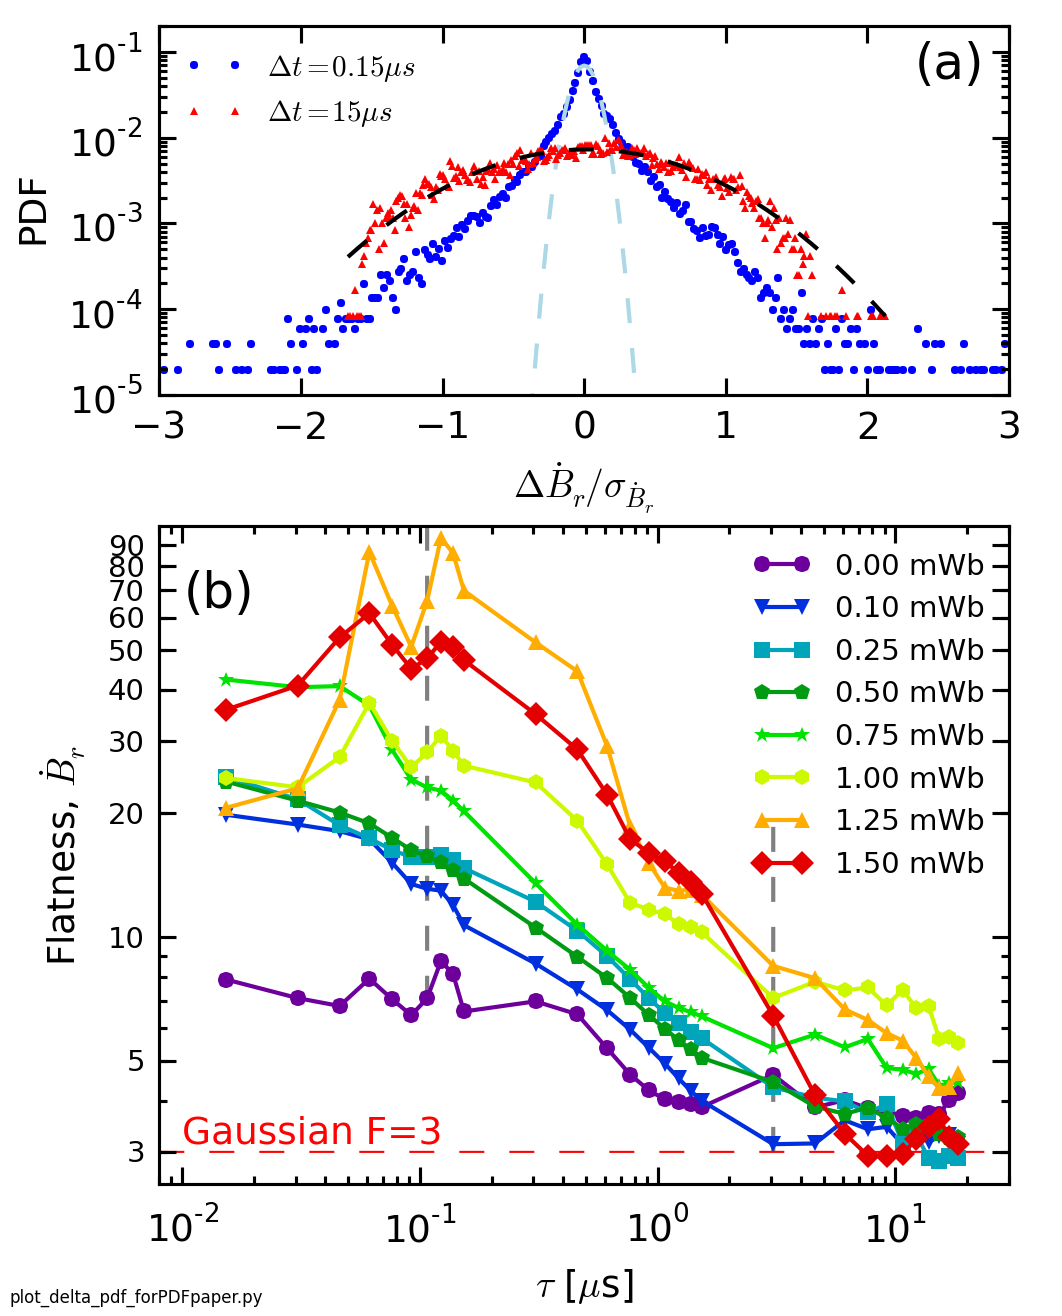
\includegraphics[width=8.5cm]{Br_flatness.png}}
\caption{\label{fig:Br_flatness} (a) PDFs for a long and short $\tau$ from data for $K_{B} = 2\times 10^{-5} Wb^{2}$ indicating the changing in intermittency with timescale. (b) Flatness values for each timescale and each helicity state for the radial $\dot{B}$ component.}
\end{figure}

This change with helicity is summarized in Figure~\ref{fig:flatness_scaling}(a) where the calculated flatness of each curve in Fig.~\ref{fig:Br_flatness}(b) as well as those for $\dot{B}_{\theta}$ and $\dot{B}_{z}$ has been averaged between the scales indicated by the dashed gray lines: between $0.1\mu s$ and $3.0\mu s$, which approximately corresponds to a frequency range of 333kHz to 10MHz. The average flatness generally increases with helicity, although there is a brief reversal of trend at about 1$\times 10^{-5}$ Wb$^{2}$ before the curve begins to increase again.

\begin{figure}[!htbp]
\centerline{
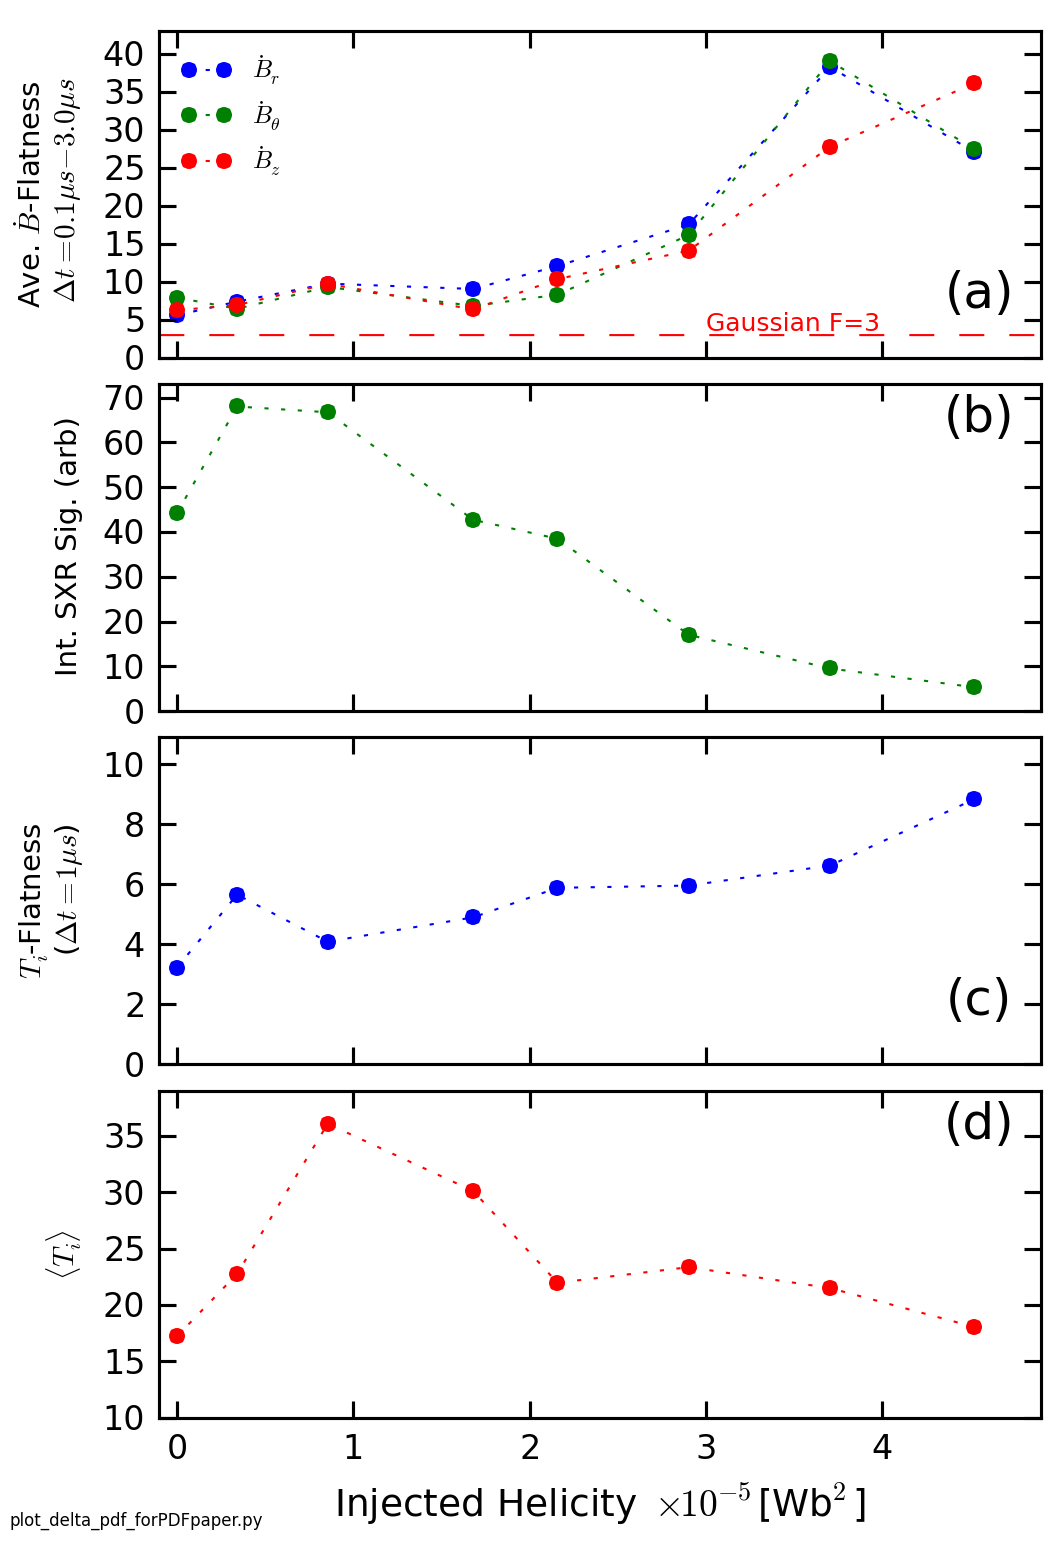
\includegraphics[width=8.5cm]{flatness_scaling.png}}
\caption{\label{fig:flatness_scaling} (a) Aveage flatness versus helicity. (b) Integrated soft X-ray signal versus helicity. (c) Flatness of $T_{i}$ time series versus helicity. (d) Average $T_{i}$ versus helicity.}
\end{figure}

While the physical origin of this observed intermittency and its trend with helicity is not completely understood in the context of this experiment, investigation of intermittency in space plasma yields some possible explanations. Simulations of MHD plasmas modeled after solar wind plasma with time series extracted in ways to match that of \textit{in-situ} satellite observation~\cite{Greco08,Servidio09,Greco09}, have indicated a correlation between intermittency and the passing of current sheets or reconnection sites. Results on SSX suggest that the appearence and change in observed intermittency can be connected to the changing size and/or frequency of reconnection sites in the plasma. Since many past experiments on SSX have focused on observation of recconection layers~\cite{SSX cites}, the machine has a number diagnostics designed to measure signatures of reconnection. These diagnostics are a set soft X-ray photodiodes and the ion doppler spectrometer (IDS) system. The soft X-ray diagnostics is designed to measure X-rays generated by fast tail electrons which were potentially accelerated in the electric field of reconnection cites. Meanwhile, the IDS can measure both burst of ion heating and flow also generated by reconnection events. Fig.~\ref{fig:flatness_scaling}(b-d) shows the output of these diagnostics for the same helicity scan limited to the same time range as the turbulence data presented above. Soft X-ray measurement shows an initial increase in x-ray light going from zero to small amounts of helicity, but then a consistent decrease in radiation from then on. Fig.~\ref{fig:flatness_scaling} shows flatness of the ion temperature timeseries as a function of helicity constructed from increment PDFs with a timescale of $1\mu s$, the minimum timestep available for the IDS system. Like, the flatness curve of $\dot{B}$, the ion curve also increases with helicity. Meanwhile, the average measured ion temperature with flatness does not change too much, peaking slightly between 1 and 2$\times 10^{-5}$ Wb$^{2}$, but generally maintaining a value of between 20-25eV. Though all of these results are somewhat circumstantial, they all fit with the hypothesis of a changing reconnection site size. The decrease in soft X-ray may perhaps be due to decreasing reconnection size as electrons cannot be accelerated to as large as velocities with smaller sites. The increase in ion temperature bursts with little change in the mean ion temperature can arise from a high frequency of recconection sites. Unlike electrons, the outflow velocity of ions is less likely to be modified by the physical size of the reconnection site. 

Unfortunately, since the reconnection diagnostics used here measure line averaged quantities, better evidence for the affect of helicity on reconnection event size cannot be determined as of yet. However, as in solar wind experiments, comparison to simulation may help and studies using the HiFi simulation are underway.

This paper presents the observation of a clear change in intermittency as a function of injected helicity while simultaneously showing little to no change in the energy transfer rate between scales as indicated by the turbulent power spectra. This discrepancy is perhaps an indication of the need to study higher order moments in turbulence analysis (i.e. 4th order Flatness vs 2nd order spectra) in order to fully flesh out modifications in turbulence. The experiment also demonstrates a straightforward method for modifying the intermittency in a plasma for detailed study. Finally, a possible connection to a physical mechanism was established through soft X-ray and IDS measurements, which suggested the intermittency is related to the spatial size of reconnection sites in the plasma. However, given the limitations of the current diagnostics, any definitative conclusions could not be made, but does provide impoteus for further comparison to simulation.

%\begin{table}
%\caption{\label{tab:params}MHD wind tunnel plasma parameters during the equilibrium epoch for the present configuration of SSX.}
%\begin{tabular}{|l|l|l|l|l|l|l|l|}
%\hline
%$V_{a}$&$f_{ci}$&Axial $\tau_{A}$&Radial $\tau_{A}$&$\rho_{i}$&$\delta_{i}$&$C_{s}$&$\beta$\\
%\hline
%$240km/s$&$7.6MHz$&3.5$\mu$s&0.3$\mu$s&0.091cm&0.51cm&31km/s&0.0967\\
%\hline
%\end{tabular}
%\end{table}

%In the equilibrium epoch, the average magnetic field is $5$kG and average density is $2\times 10^{15}$cm$^{-3}$; thus, radial and axial Alfv\'en transit times are $0.3\mu$s and $3.5\mu$s respectively. Ion temperature is measured using an ion Doppler spectrometer system at the midplane. Background ion temperatures (i.e. average temperatures made avoiding large heating events) are on the order of $20$eV. Though not measured in this dataset, previous measurements of the electron temperature suggest a value of $10$eV for this system. Combined with the average field and density values measured, estimates of ion gyrofrequency ($f_{ci}$), ion gyroradius ($\rho_{i}$) and ion inertial length ($\delta_{i}$) can be made. These values are listed in Table~\ref{tab:params}. Of particular note, the ratio of system size to $\rho_{i}$ is large, $R/\rho_{i} \cong 80$, suggesting that the influence of the wall on plasma dynamics is minimal.

%The density trace in Figure~\ref{fig:timeseries36}(b) shows peaking in the formation epoch, but an eventual drop to approximately $10^{15}$cm$^{-3}$ for the majority of the discharge. The initial peaking is likely due to the initial spheromak formation, where plasma is being pushed into the tunnel, but before the threshold for break-off is achieved. The Mach number trace is on average positive, indicating flow predominately away from the gun source as would be expected for a single source configuration. The average Mach number during the equilibrium epoch is $M=0.4$ which for the sound speed $C_s$ listed in Table~\ref{tab:params} yields an average flow speed of $12$km/s. It is likely that flow speeds toward the center can be even higher. Indeed, a time of flight estimate based on the axial separation distance between the interferometer measurement and the midplane $\dot{B}$ measurement suggests a bulk plasma flow of $20$km/s. As seen in the single shot trace in Figure~\ref{fig:timeseries36}, there can sometimes be a flow reversal which likely indicates a reflection of flow off of the far axial boundary.

%It can also be observed that the decay times for the magnetic field and the Mach number, during the dissipation epoch, are on the same order. This suggests a Prandtl number of $O(1)$. That is, resistive and viscous effects are on the same order for these discharges.

%Given the dynamical nature of these plasmas, the spectral decomposition has been achieved using a Wavelet technique rather than with Fast Fourier Transforms (FFTs). This wavelet technique has been shown to be useful in situations where data may be non-stationary and provides a more accurate method for simultaneous spectral and temporal decomposition than a windowed Fourier transform because it applies a transform at many scales rather than a single scale~\cite{torrence98}. To achieve better resolution in frequency space, a sixth-order Morlet mother wavelet has been used. Morlet wavelet scales (i.e. frequencies) are generally well matched to Fourier scales, though it has also been shown that the choice of wavelet is not critical for determining power spectral densities (PSD)~\cite{torrence98}. A wavelet decomposition for a single shot $\dot{B}$ time-series is shown in Figure~\ref{fig:waveletcontour} with the wavelet scale converted to a Fourier frequency as the $y$-axis and time as the $x$-axis. The color scale corresponds to the normalized fluctuation power. Changes in the spectral nature can be seen with time: higher frequency fluctuations grow up and peak around $30\mu$s, hold stable until about $60\mu$s, and then begin to dissipate. This change in fluctuations supports the division of the data into epochs.

%The reduced power spectra for B-field, density and Mach number fluctuations are displayed in Figure~\ref{fig:waveletspec}. The B-field curves are produced by first taking a wavelet transform of the $\dot{B}$ time-series (for any one of the orthogonal components), yielding an array with $\dot{B}$ fluctuation power as a function of both time and frequency as in Figure~\ref{fig:waveletcontour}, and scaling the $\dot{B}$ power by $f^{2}$ in order to recover actual B-field fluctuation power. This approach is derived from the assumption that the B-field fluctuations can be Fourier decomposed such that
%
%\begin{equation}
%\frac{d}{dt}B(t) = \frac{d}{dt}B_{0}e^{i2\pi f} \sim ifB
%\end{equation}
%
%resulting in the relationship between $\tilde{B}(f)$ and $\tilde{\dot{B}}(f)$ as
%
%\begin{equation}
%|\tilde{B}(f)|^{2} = \frac{1}{f^{2}}|\tilde{\dot{B}}(f)|^{2}
%\end{equation}
%
%where $|\tilde{x}(f)|^{2}$ is the PSD. The same relationship applies for the Wavelet Transform. Once converted into a B-field power array, the 1D spectrum is calculated by summing over a certain time region - in this case the equilibrium epoch of $40\mu$s to $60\mu$s. The shot-averaged spectra for the magnetic field components ($B_{r}$, $B_{\theta}$, $B_{z}$) are nearly identical suggesting that magnetic fluctuations are isotropic. For clarity, only the $B_{\theta}$ component is shown in Figure~\ref{fig:waveletspec}.  A similar approach is taken for density and Mach number, though without the frequency scaling.

%All three curves shown have roughly linear behavior in the spectral region between $50$kHz and $10$MHz. A power-law fit of spectral power to frequency ($P(f) \sim f^{-\alpha}$) is made for density and Mach number in this frequency range using a maximum likelihood estimation method (MLE)~\cite{clauset09} yielding exponents of $\alpha = 1.57$ for the density spectrum and $\alpha = 1.62$ for the Mach spectrum, which serves as a proxy for the velocity spectrum in this experiment. An exponent of $1.62$ for velocity is very close to the typical Kolmogorov exponent of $5/3 = 1.66$ for hydrodynamic flow fluctuations.

%The magnetic field spectrum appears to have two separate regions: a shallower sloped region between $50$kHz and $1$MHz and a steeper sloped region between $1$MHz and $10$MHz. MLE fits for these regions give exponents of $\alpha = 2.47$ (shallower) and $\alpha = 4.36$ (steeper). Both the plots and the fits indicate that the spectra index for B-field fluctuations is steeper than that for Mach (velocity) fluctuations and thus steeper than that measured in the solar wind. This is perhaps indicative of a magnetic field dissipation mechanism that is present in the experimental plasma, but not in space.

%The origin of the break in the spectra may come about in a number of ways. First, it may simply be due to the effect of flowing plasma across the probe. The Taylor hypothesis - frozen-in flow - suggests that measured temporal spectra can be mapped to spatial spectra when the medium containing the fluctuations is moving past a probe at some velocity. Thus, in the spectrum, there is some critical frequency below which fluctuations can be considered to be predominately due to spatial structure, and above which fluctuations are due to some combination of spatial and temporal structure. A rough estimate for this critical frequency can be made by considering the average flow and probe size. The average axial flow for the equilibrium epoch as indicated by the Mach probe and the assumed $C_s$ is $12$km/s; with a $3$mm probe size, the critical frequency would be $4$MHz. Thus, the break in the slope could be showing a transition between the power spectrum representing the energy transfer in both spatial and temporal scales (higher frequencies) and a spectrum due to the energy transfer in only spatial scales (lower frequencies), since lower frequency temporal fluctuations become less observable by the probe. 

%The break could also be related to the temporal decorrelation of the signal. Figure~\ref{fig:autocorr} shows the autocorrelation function for $\dot{B}$ for each of the three axes, again during the equilibrium epoch. A decorrelation time can be defined as the $\tau$ at which the autocorrelation function crosses zero. For $\dot{B}_{r}$ and $\dot{B}_{\theta}$, $\tau = 1.0\mu$s which corresponds to a frequency of $1$MHz - also called a decorrelation rate. If there are any wave modes in the plasma, they could influence the spectrum at frequencies below the decorrelation rate. Indeed, there has been some evidence that mode types can have an effect on energy transfer rates that manifest in the power spectrum~\cite{shaikh09}. Above the decorrelation rate, the fluctuations arise purely from the turbulence which may have a different energy transfer rate. Consequently, this may appear as a change in the spectral index around the decorrelation frequency.

%Finally, this break may be due, of course, to a transition to the dissipation range of the spectrum. Possible dissipation scales include the ion gyroradius and ion inertial lengths which are $\sim 0.1$cm and $\sim 0.5$cm, respectively, for the equilibrium epoch. Dissipation could also occur directly in frequency space with coupling to the ion gyrofrequency, which here is $7.6$MHz. If the Taylor hypothesis is made, and frequencies are mapped to wavelengths using the average velocity, the break point occurs at a length of $1.2$cm; the ion inertial length scale maps to a frequency of $2.4$MHz.

%Synthetic diagnostics of the HiFi simulations of the SSX MHD wind tunnel also produce time series B-field, density and flow measurements, with the diagnostics location and probe sizes designed to resemble those used in the experiment as much as possible. For example, B-field at the mid-plane is measured by taking a volume average over a $0.3$cm diameter sphere corresponding to the size of the experimental probes; while the axial location of the chord-averaged plasma number density diagnostic, as well as the radial location of the mid-plane flow measurement, correspond to the locations of the respective experimental measurements.  However, unlike the experimental data, the simulated discharge consists of only a single spheromak that undergoes expansion, Taylor relaxation and decay with a lifetime on the order of $50\mu$s. The simulation does not presently model slow formation, or the sustainment of plasma injection seen in the experiment; however, a comparison between the two can be made by observing the similarity of the simulated pulse with the tail end of the experimental discharge. This can be clearly seen in Figure~\ref{fig:simtimeseries64} where the simulated time series has been shifted to approximately match the decay features of the B-field, as well as few fluctuation features of the density and Mach number. The experimental shot shown in Figure~\ref{fig:simtimeseries64} was chosen for its particularly well-matched features.

%This similarity highlights the assertion that despite the longer injection time of plasma in the experiment (and thus, less well-defined large scale structure), the selective decay and self-organization still occurs. Moreover, the similarity allows us to compare the turbulent features of the experiment and the HiFi simulations.

%Figure~\ref{fig:simBspectra} shows wavelet spectra for the simulation runs as well as the averaged experimental spectra. Due to the smaller number of points in the simulation time-series, the wavelet decomposition used a fourth-order Paul mother wavelet, which has a slightly better time resolution than the sixth-order Morlet wavelet used above. The experimental data is also reanalyzed using the Paul wavelet for direct comparison to the simulation data. (Note that the differences between the two wavelet transforms is minimal for the experimental data, which is sampled at a higher frequency.) Like the experimental spectra, there appear to be two linear regions in the simulation spectra. The slopes of both the resistive-MHD and Hall-MHD simulation spectra are very close to that of the experimental data in the region between $20$kHz and $300$kHz. The simulation spectra, however, begin to steepen at a lower frequency than the experimental data: $\sim 300$kHz compared to $\sim 1$MHz. This is consistent with the autocorrelation function for the simulation which gives decorrelation times on the order of $3.3\mu$s. The simulations do not appear to shed any light on the possible role of dissipation. The spectra for both resistive-MHD and Hall-MHD simulations are similar, so that any modification of the underlying dynamics due to the inclusion of the Hall physics is not apparent in the data. Nevertheless, the slope of the simulation spectra are very close to the experiment.
%Speculation about ion inertial length with Hall term simulation? 

%While spectra can be useful for obtaining the relative rate of energy transfer amongst injection, inertial and dissipation scales, they can obscure other signatures of turbulence that can only be seen when looking at higher integral moments. One technique for investigating these higher moments is to construct probability distribution functions (PDFs) from the data at different timescales and then to directly calculate the moments. The variation in the moments of PDFs as a function of timescale has been shown to be linear for fully-developed fluid turbulence~\cite{frisch95}. One can introduce a timescale into the time-series by filtering~\cite{frisch95,wan12} or by taking differences of the data points at different time steps~\cite{Greco08,Greco09}. This latter technique is used here, where a series of $\Delta\dot{B}$ increments is constructed for a variety of timesteps, $\tau$, as in
%\begin{equation}
%\Delta \dot{B}_{\tau}(t) = \dot{B}(t+\tau)-\dot{B}(t)
%\label{eq:increments}
%\end{equation}

%\begin{figure}[!htbp]
%\centerline{
%\includegraphics[width=8.5cm]{figure8a_8d.eps}}
%\caption{\label{fig:pdfs} PDFs of $\Delta \dot{B}$ in the time range 40 to 60 $\mu$s normalized to the standard deviation for each list and total integral of the histogram for different time increments: (a) $0.15\mu s$, (b) $0.75\mu s$, (c) $3.00\mu s$ and (d) $15.0\mu s$.}
%\end{figure}
%\begin{figure}[!htbp]
%\centerline{
%\includegraphics[width=8.5cm]{figure9.eps}}
%\caption{\label{fig:flatness} The flatness of the PDFs as a function of $\tau$ on a log-log scale. A flatness of $3$ would indicate a perfectly Gaussian distribution. A linear slope between $0.1\mu$s and $1\mu$s - corresponding to the frequency range of $1$MHz to $10$MHz - suggests a power-law like relationship between the flatness and the timestep. The flatness curves for the HiFi simulations are also listed. They show a similar shape, but offset in $\tau$.}
%\end{figure}

%A series of these PDFs for the equilibrium epoch time-series is shown in Figure~\ref{fig:pdfs} for $\tau$'s of $0.15\mu$s, $0.75\mu$s, $3\mu$s and $15\mu$s which corresponds to filtering the time-series above frequencies of $6.6$MHz, $1.3$MHz, $333$kHz, and $66$kHz respectively. The PDFs are normalized to the root mean square value of the increments and to the total integral of the histogram. A Gaussian function is fit to each distribution. One can clearly see a transition from non-Gaussian distributions for small $\tau$'s to more Gaussian distribution for larger $\tau$'s. The features of the non-Gaussian distributions are indicative of intermittency in the signal; the fat tails signify large swings in the values of the time-series and the timestep indicates the relative temporal size of the intermittent events.

%The level of intermittency as a function of $\tau$ can be quantified using a calculation of the flatness defined as~\cite{deWit13}
%\begin{equation}
%F(\tau) = \frac{S_{4}(\tau)}{S_{2}(\tau)^{2}}
%\label{eq:flatness}
%\end{equation}
%where $S_{p}(\tau)$ is the $p^{th}$ order moment for the distribution of increments, $\Delta \dot{B}$, as in
%\begin{equation}
%S_{p}(\tau) = \int_{-x_{max}}^{x_{max}} P(\Delta \dot{B})(\Delta \dot{B})^{p} dx
%\label{eq:structurefunc}
%\end{equation}
%with $x$ representing a histogram bin width. An exact Gaussian distribution would have a flatness equal to $3$.

%The resulting function for flatness is shown in Figure~\ref{fig:flatness} for each of the three $\dot{B}$ measurements. The plot shows the trend toward Gaussian (as represented by the dashed line at $F=3$) as the timestep is increased. An increase in flatness signifies an increase in the intermittency observed in the PDF - the flatness grows rapidly beyond $\tau = 1\mu$s corresponding to a frequency of $1$MHz. Since fluctuations beyond this frequency are more and more temporally correlated (as indicated by the autocorrelation function), it is clear that the intermittent nature is truly embedded in the magnetic signal. Conversely, a trend toward a Gaussian distribution might be expected for fluctuations that are not temporally correlated; however, recent work in this vein on solar wind measurements has speculated that such a change in flatness versus timescale might be expected at the transition from inertial to dissipation range turbulence~\cite{wan12}. It is also worth noting that the transition occurs around the autocorrelation time measured above. This is perhaps not unlike the spatial PDF measurement conducted in Greco, {\it et al}~\cite{Greco08} which showed a tendency toward Gaussian distributions beyond the radial correlation length whose analogue here would be the autocorrelation time.

%The simulation data can also be analyzed within the PDF of increments framework. The flatness curve is also shown in Figure~\ref{fig:flatness} for the two different simulation runs. The shape of the curve is very similar to the experimental one, though the changes in flatness are offset in time increment as higher values of flatness are reached at larger increments. The largest values of flatness for both the experiment and the simulation are similar, suggesting that the mechanism responsible for the intermittency might be common to both.

%We have hypothesized that the turbulent relaxation of a twisted flux rope plasma in the SSX wind tunnel was promoted by intermittency and coherent structures.  The rapidity of the relaxation process (about one Alf\'ven time) could be due to fast local relaxation of the coherent structures followed by a slower relaxation of the structure as a whole.  In this study, we have focused on time series and temporal frequency statistics: autocorrelation function, power frequency spectra, and PDFs of temporal increments.  Spatial correlations and spectra will be reported in a later article.

%Magnetic field power frequency spectra from the experiment show power-law behavior over two decades but with steeper spectral indices than measured in the solar wind and predicted from theory. Comparisons of power frequency spectra with numerical simulations show good correspondence with indices $\alpha \approx 2.5$ at low frequencies and steeper at higher frequencies.  The reason for the break in the spectra slope has not been identified; however, both experimental and simulation data had measured decorrelation rates which could be placed near the respective break points. Furthermore, it is not clear whether a dissipation scale has been observed in the SSX plasma in these experiments.

%Probability distribution functions of the magnetic field increments expose non-Gaussian higher order statistics connected to intermittency and coherent structures.  We find large values of flatness at short time increments corresponding to small spatial scales in both the experiment and the simulations.  In addition, we find that the shape of the curve of flatness with increasing time increment is also very similar in both the experiment and the simulations.

%The observation of non-Gaussian values for flatness in the PDFs, and the trend for increasing flatness with decrease in timestep is a strong indication for the presence of intermittent fluctuations and/or coherent structures in the plasma, which could not be observed with spectra alone. The physical origin of these coherent structures in the SSX plasma has not yet been identified. As seen in previous simulation work~\cite{Servidio11b}, the coherent structures can be matched to the presence of current sheets which in turn could be the site of a reconnection layer. Given the observation of reconnection in past SSX work~\cite{Cothran09,Gray10}, there is a strong likelihood that such events are present in the current SSX configuration though perhaps at a smaller scale.

% ----------------------------------------------------------------
\section*{Acknowledgements}
%  We gratefully acknowledge many useful discussions with William Matthaeus. This work has been funded by the US DoE Experimental Plasma Research program and the National Science Foundation.  The simulations were performed using the advanced computing resources (Cray XC30 Edison system) at the National Energy Research Scientific Computing Center.
% ----------------------------------------------------------------
\section*{References}
\begin{thebibliography}{10}
\bibitem{Oieroset11}
Oieroset, M., {\it et al.} Direct evidence for a three-dimensional magnetic flux rope flanked by two active magnetic reconnection X-lines at the Earth's magnetopause, Phys. Rev. Lett. {\bf 107}, 165007, (2011).
%Oieroset, M., T. D. Phan, J. P. Eastwood, M. Fujimoto, W. Daughton, M. Shay, V. Angelopoulos, F. S. Mozer, J. P. McFadden, D. E. Larson, and K. -H. Glassmeier, Direct evidence for a three-dimensional magnetic flux rope flanked by two active magnetic reconnection X-lines at the Earth's magnetopause, Phys. Rev. Lett. {\bf 107}, 165007, (2011).

\bibitem{Patsourakos13}
S. Patsourakos, A. Vourlidas, and G. Stenborg. Direct Evidence for a Fast Coronal Mass Ejection Driven by the Prior Formation and Subsequent Destabilization of a Magnetic Flux Rope, ApJ {\bf 764}, 125, (2013).
%S. Patsourakos, A. Vourlidas, and G. Stenborg. Direct Evidence for a Fast Coronal Mass Ejection Driven by the Prior Formation and Subsequent Destabilization of a Magnetic Flux Rope, ApJ {\bf 764}, 125, (2013).

\bibitem{Gray13} 
T. Gray, M. R. Brown, and D. Dandurand, Observation of a Relaxed Plasma State in a Quasi-Infinite Cylinder, Phys. Rev. Lett. {\bf 110}, 085002 (2013). 

\bibitem{Taylor86} J. B. Taylor, Rev. Mod. Phys. {\bf 58}, 741 (1986).

\bibitem{Matthaeus80} W.H. Matthaeus and D. Montgomery, Ann. N.Y. Acad. Sci. {\bf 357}, 203 (1980).

\bibitem{Servidio08}
Servidio, S., Matthaeus, W. H., and Dmitruk, P.: Depression of Nonlinearity in Decaying Isotropic MHD Turbulence, Phys. Rev. Lett. {\bf 100}, 095005 (2008).

\bibitem{Servidio11}
Servidio, S., Dmitruk, P., Greco, A., Wan, M., Donato, S., Cassak, P. A., Shay, M. A., Carbone, V., Matthaeus, W. H., Magnetic reconnection as an element of turbulence, Nonlin. Processes Geophys. {\bf 18}, 675-695 (2011). 

\bibitem{Servidio09}
Servidio, S., Matthaeus, W. H., Shay, M. A., Cassak, P. A., and Dmitruk, P.: Magnetic Reconnection in Two-Dimensional Magnetohydrodynamic Turbulence, Phys. Rev. Lett. {\bf 102}, 115003 (2009).

\bibitem{Servidio10a}
Servidio, S., Matthaeus, W. H., Shay, M. A., Dmitruk, P., Cassak, P. A., and Wan, M.: Statistics of magnetic reconnection in two- dimensional magnetohydrodynamic turbulence, Phys. Plasmas {\bf 17}, 032315 (2010).

\bibitem{Greco08}
A. Greco, P. Chuychai, W. H. Matthaeus, S. Servidio and P. Dmitruk, Intermittent MHD structures and classical discontinuities, Geophys. Res. Lett. {\bf 35}, L19111 (2008).

\bibitem{Greco09}
Greco, A., Matthaeus, W. H., Servidio, S., Chuychai, P., and Dmitruk, P.: Statistical Analysis of Discontinuities in Solar Wind ACE Data and Comparison with Intermittent MHD Turbulence, ApJ {\bf 691}, L111 (2009).

\bibitem{Wan09}
Wan, M., Oughton, S., Servidio, S., and Matthaeus, W. H.: Generation of non-Gaussian statistics and coherent structures in ideal magnetohydrodynamics, Phys. Plasmas {\bf 16}, 080703 (2009).

\bibitem{Lukin11}
V.~S. Lukin and M.~G. Linton.
\newblock Three-dimensional magnetic reconnection through a moving magnetic null.
\newblock \emph{Nonlin. Processes Geophys.}, 18:\penalty0 871--882, 2011.

\bibitem{jarboe83}
T. R. Jarboe, I. Henins, A. R. Sherwood, Cris W. Barnes, and H. W. Hoida, Slow Formation and Sustainment of Spheromaks by a Coaxial Magnetized Plasma Source, Phys. Rev. Lett. {\bf 51}, 39�42 (1983).

\bibitem{Zhang11}
X. Zhang, D. Dandurand, T. Gray, M. R. Brown, and V. S. Lukin, Calibrated Cylindrical Mach Probe in a Plasma Wind Tunnel, Rev. Sci. Instr. {\bf 82}, 033510 (2011).

\bibitem{Glasser04}
A.~H. Glasser and X.~Z. Tang.
\newblock The {SEL} macroscopic modeling code.
\newblock \emph{Comp. Phys. Comm.}, 164:\penalty0 237, 2004.

\bibitem{Lukin08}
V.~S. Lukin.
\newblock \emph{Computational study of the internal kink mode evolution and associated magnetic reconnection phenomena}.
\newblock PhD thesis, Princeton University, 2008.

\bibitem{Chodura75}
R.~Chodura.
\newblock A hybrid fluid-particle model of ion heating in high-mach-number shock waves.
\newblock \emph{Nucl. Fusion}, 15:\penalty0 55, 1975.

\bibitem{Sgro76}
A.~G. Sgro and C.~W. Nieslon.
\newblock Hybrid model studies of ion dynamics and magnetic field diffusion during pinch implosions.
\newblock \emph{Phys. Fluids}, 19:\penalty0 126--133, 1976.

\bibitem{Meier11}
E.~T. Meier.
\newblock \emph{Modeling Plasmas with Strong Anisotropy, Neutral Fluid Effects, and Open Boundaries}.
\newblock PhD thesis, University of Washington, 2011.

\bibitem{Krall86}
N.~A. Krall and A.~W. Trivelpiece.
\newblock \emph{Principles of Plasma Physics}, chapter Chapter 6: Transport Phenomena in Plasma, pages 311--317.
\newblock San Francisco Press, Inc., 1986.

\bibitem{torrence98}
C. Torrence, G.P. Compo, A practical guide to wavelet analysis. Bull. Am. Meteorol. Soc. {\bf 79}, 6178 (1998).

\bibitem{clauset09}
A. Clauset, C. Rohilla Shalizi, M.E.J. Newman, Power-law distributions in empirical data, SIAM Rev. {\bf 51}, 661703 (2009).

\bibitem{shaikh09}
D. Shaikh and P.K. Shukla, 3D Simulations of Fluctuation Spectra in the Hall-MHD Plasma, Phys. Rev. Lett. {\bf 102}, 045004 (2009).

\bibitem{frisch95}
Frisch, U. 1995, {\it Turbulence} (Cambridge: Cambridge Univ. Press)

\bibitem{wan12}
M. Wan, K. T. Osman, W. H. Matthaeus, and S. Oughton, Investigation of intermittency in magnetohydrodynamics and solar wind turbulence: scale-dependent kurtosis, ApJ {\bf 744}, 171 (2012).

\bibitem{deWit13}
T. Dudok de Wit, O. Alexandrova, I. Furno, L. Sorriso-Valvo, G. Zimbardo, Methods for Characterising Microphysical Processes in Plasmas, Space Sci. Rev. {\bf 0038-6308}, p. 1-29 (2013).

\bibitem{Servidio11b}
Servidio, S., Greco, A., Matthaeus, W. H., Osman, K. T., and Dmitruk, P.: Statistical association of discontinuities and reconnection in magnetohydrodynamic turbulence, J. Geophys. Res. {\bf 116}, A09102 (2011).

\bibitem{Cothran09}
C. D. Cothran, M. R. Brown, T. Gray, M. J. Schaffer, and G. Marklin, Phys. Rev. Lett. {\bf 103}, 215002 (2009).

\bibitem{Gray10}
T. Gray, V. S. Lukin, M. R. Brown, C. D. Cothran, Three-dimensional reconnection and relaxation of merging spheromak plasmas, Phys. Plasmas {\bf 17}, 102106 (2010).

\bibitem{carter06}
T.A. Carter, Intermittent turbulence and turbulent structures in a linear magnetized plasma, Phys. Plasmas 13, 010701 (2006)

\bibitem{serianni07}
G Serianni et al 2007 Plasma Phys. Control. Fusion 49 B267

\end{thebibliography}

\end{document}

